\documentclass{beamer}
\usetheme{PaloAlto}
\usepackage{url}
\usepackage{latexsym}
\usepackage{graphicx}


% My Package Includes
\usepackage{upquote} % For real apostrophes (see http://tex.stackexchange.com/questions/63345/how-to-make-a-real-apostrophe-or-single-quote-in-latex#63348)
\usepackage{comment}
\usepackage{xcolor}
\definecolor{dark-blue}{rgb}{0.15,0.15,0.7}
\usepackage{hyperref}
%\hypersetup{colorlinks, linkcolor={dark-blue}, citecolor={dark-blue}, urlcolor={dark-blue}}
\hypersetup{colorlinks, linkcolor=black, citecolor=black, urlcolor=black}
\usepackage{booktabs}
\frenchspacing % Normal (single) spaces after periods.  Cf. http://www.read.seas.harvard.edu/~kohler/latex.html
%\usepackage{natbib}
\usepackage[shortcuts]{extdash} % use "\-/" to help LaTeX insert hyphen/pagebreaks
\usepackage[textwidth=0.9in]{todonotes}
\newcommand{\smalltodo}[2][]
    {\todo[caption={#2}, #1]
    {\tiny#2\normalsize}}


\newtheorem{requirement}{Requirement}

\usepackage{glossaries}
\glossarystyle{tree}
\makeglossaries



\newacronym{api}{API}{application programming interface}
\newacronym{http}{HTTP}{Hypertext Transfer Protocol}
\newacronym{gui}{GUI}{graphical user interface}
\newacronym{ui}{UI}{user interface}
\newacronym{cl}{CL}{computational linguistics}
\newacronym{nlp}{NLP}{Natural Language Processing}
\newacronym{sil}{SIL}{Summer Institute of Linguistics}
\newacronym{json}{JSON}{JavaScript Object Notation}
\newacronym{npm}{NPM}{Node Package Manager}
\newacronym{bdd}{BDD}{behavior-driven development}
\newacronym{scrud}{SCRUD}{search, create, read, update, and delete}
\newacronym{rdbms}{RDBMS}{relational database management system}
\newacronym{igt}{IGT}{interlinear glossed text}
\newacronym{fst}{FST}{finite-state transducer}
\newacronym{cs}{CS}{context-sensitive}
\newacronym{lm}{LM}{language model}
\newacronym{url}{URL}{uniform resource locator}
\newacronym{tsv}{TSV}{tab-separated values}
\newacronym{tlg}{TLG}{Teach and Learn with Georgia}
\newacronym{flex}{FLEx}{FieldWorks Language Explorer}


\setbeamertemplate{theorem begin}{{
\inserttheoremheadfont
\inserttheoremname
\inserttheoremnumber
\ifx\inserttheoremaddition\@empty\else\ \inserttheoremaddition \fi%
\inserttheorempunctuation
}}
\setbeamertemplate{theorem end}{}


\begin{document}



\title[LingSync \& OLD] % (optional, use only with long paper titles)
{LingSync \& the Online Linguistic Database}



\author[~]{Joel Dunham \inst{1} \and Gina Cook \inst{2} \and Josh Horner \inst{3}}
\institute[UBC, LingSync.org]{\inst{1} University of British Columbia \and %
                      \inst{2} iLanguage Lab \and %
                      \inst{3} Amilia}


                      \subtitle
                      {New models for the collection and management of data for language communities, linguists and
                      language learners}

%\author[Author1,Author2] % (optional, use only with lots of authors)
%{Author One  \and Author Two }
% - Give the names in the same order as the appear in the paper.
% - Use the \inst{?} command only if the authors have different
%   affiliation.

% - Use the \inst command only if there are several affiliations.
% - Keep it simple, no one is interested in your street address.

\date[ComputEL 2014] % (optional, should be abbreviation of conference name)
{ComputEL Workshop, June 26 2014\\52nd Annual Meeting of the Association for Computational Linguistics }



% \AtBeginSubsection[]
% {
% \setbeamertemplate{sidebar left}{}
%   \begin{frame}<beamer>
%     \frametitle{Outline}
%     \tableofcontents[currentsection,currentsubsection]
%   \end{frame}
%   \setbeamertemplate{sidebar left}[sidebar theme]
%
% }

\setbeamertemplate{sidebar left}{}
\begin{frame}
\titlepage
\end{frame}
\setbeamertemplate{sidebar left}[sidebar theme]

\section{Background}

\subsection[Fieldwork]{Endangered languages fieldwork}\label{sec:fieldwork}

%\begin{frame}
%TODO Joel Endangered languages fieldwork
%\note{Joel presents}
%\end{frame}



\begin{frame}
%TODO will convert into latex diagrams once we are sure we want it.
\begin{figure}
\begin{center}
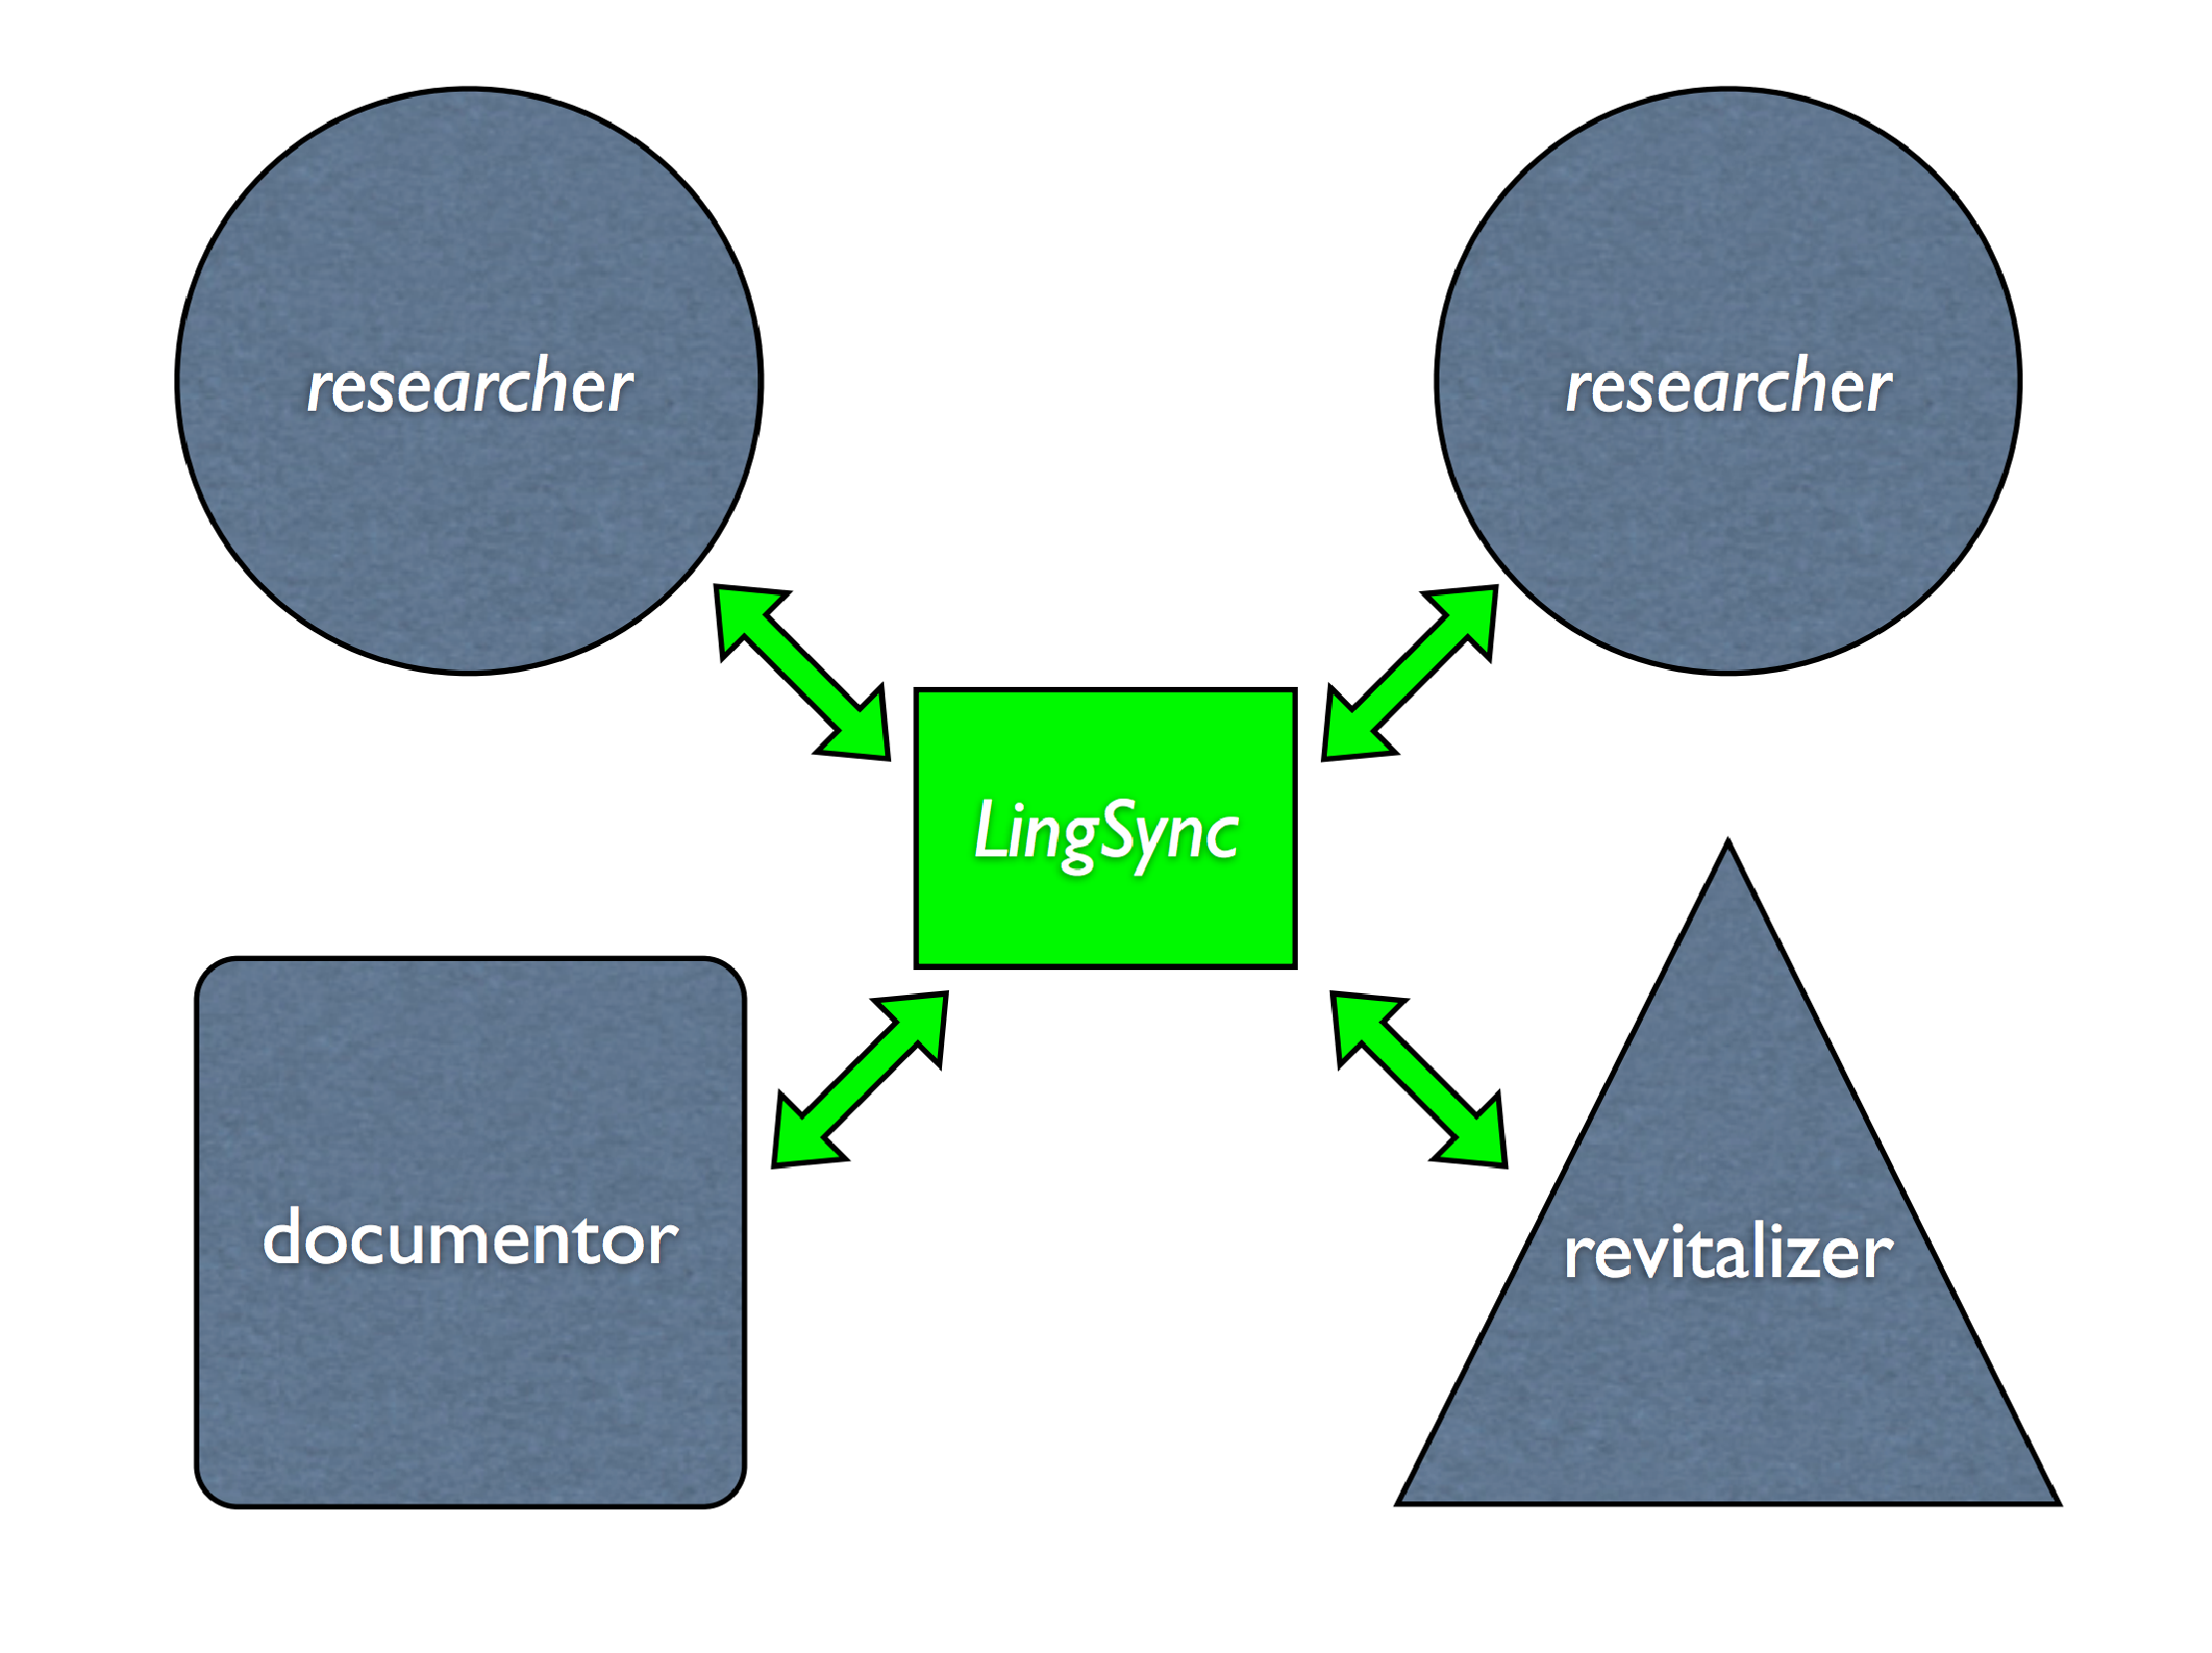
\includegraphics[width=3in]{../figures/bridge_stakeholders}
\label{lingsync:bridge}
\end{center}
\end{figure}
\note{Joel presents}
\end{frame}


\subsection[Requirements]{Software requirements}

\begin{frame}


\begin{requirement}
\label{req:primary-data}
Integration of primary data
\end{requirement}


\begin{requirement}
\label{req:curation}
Curation of data
\end{requirement}


\begin{requirement}
\label{req:inclusive}
Inclusion of stakeholders
\end{requirement}

\begin{requirement}
\label{req:openable}
Openable data
\end{requirement}


\begin{requirement}
\label{req:productivity}
User productivity
\end{requirement}

\note{Joel presents}
\end{frame}


\subsection{Existing software}

\begin{frame}


%TODO will convert into latex diagrams once we are sure we want it.
\begin{figure}
\begin{center}
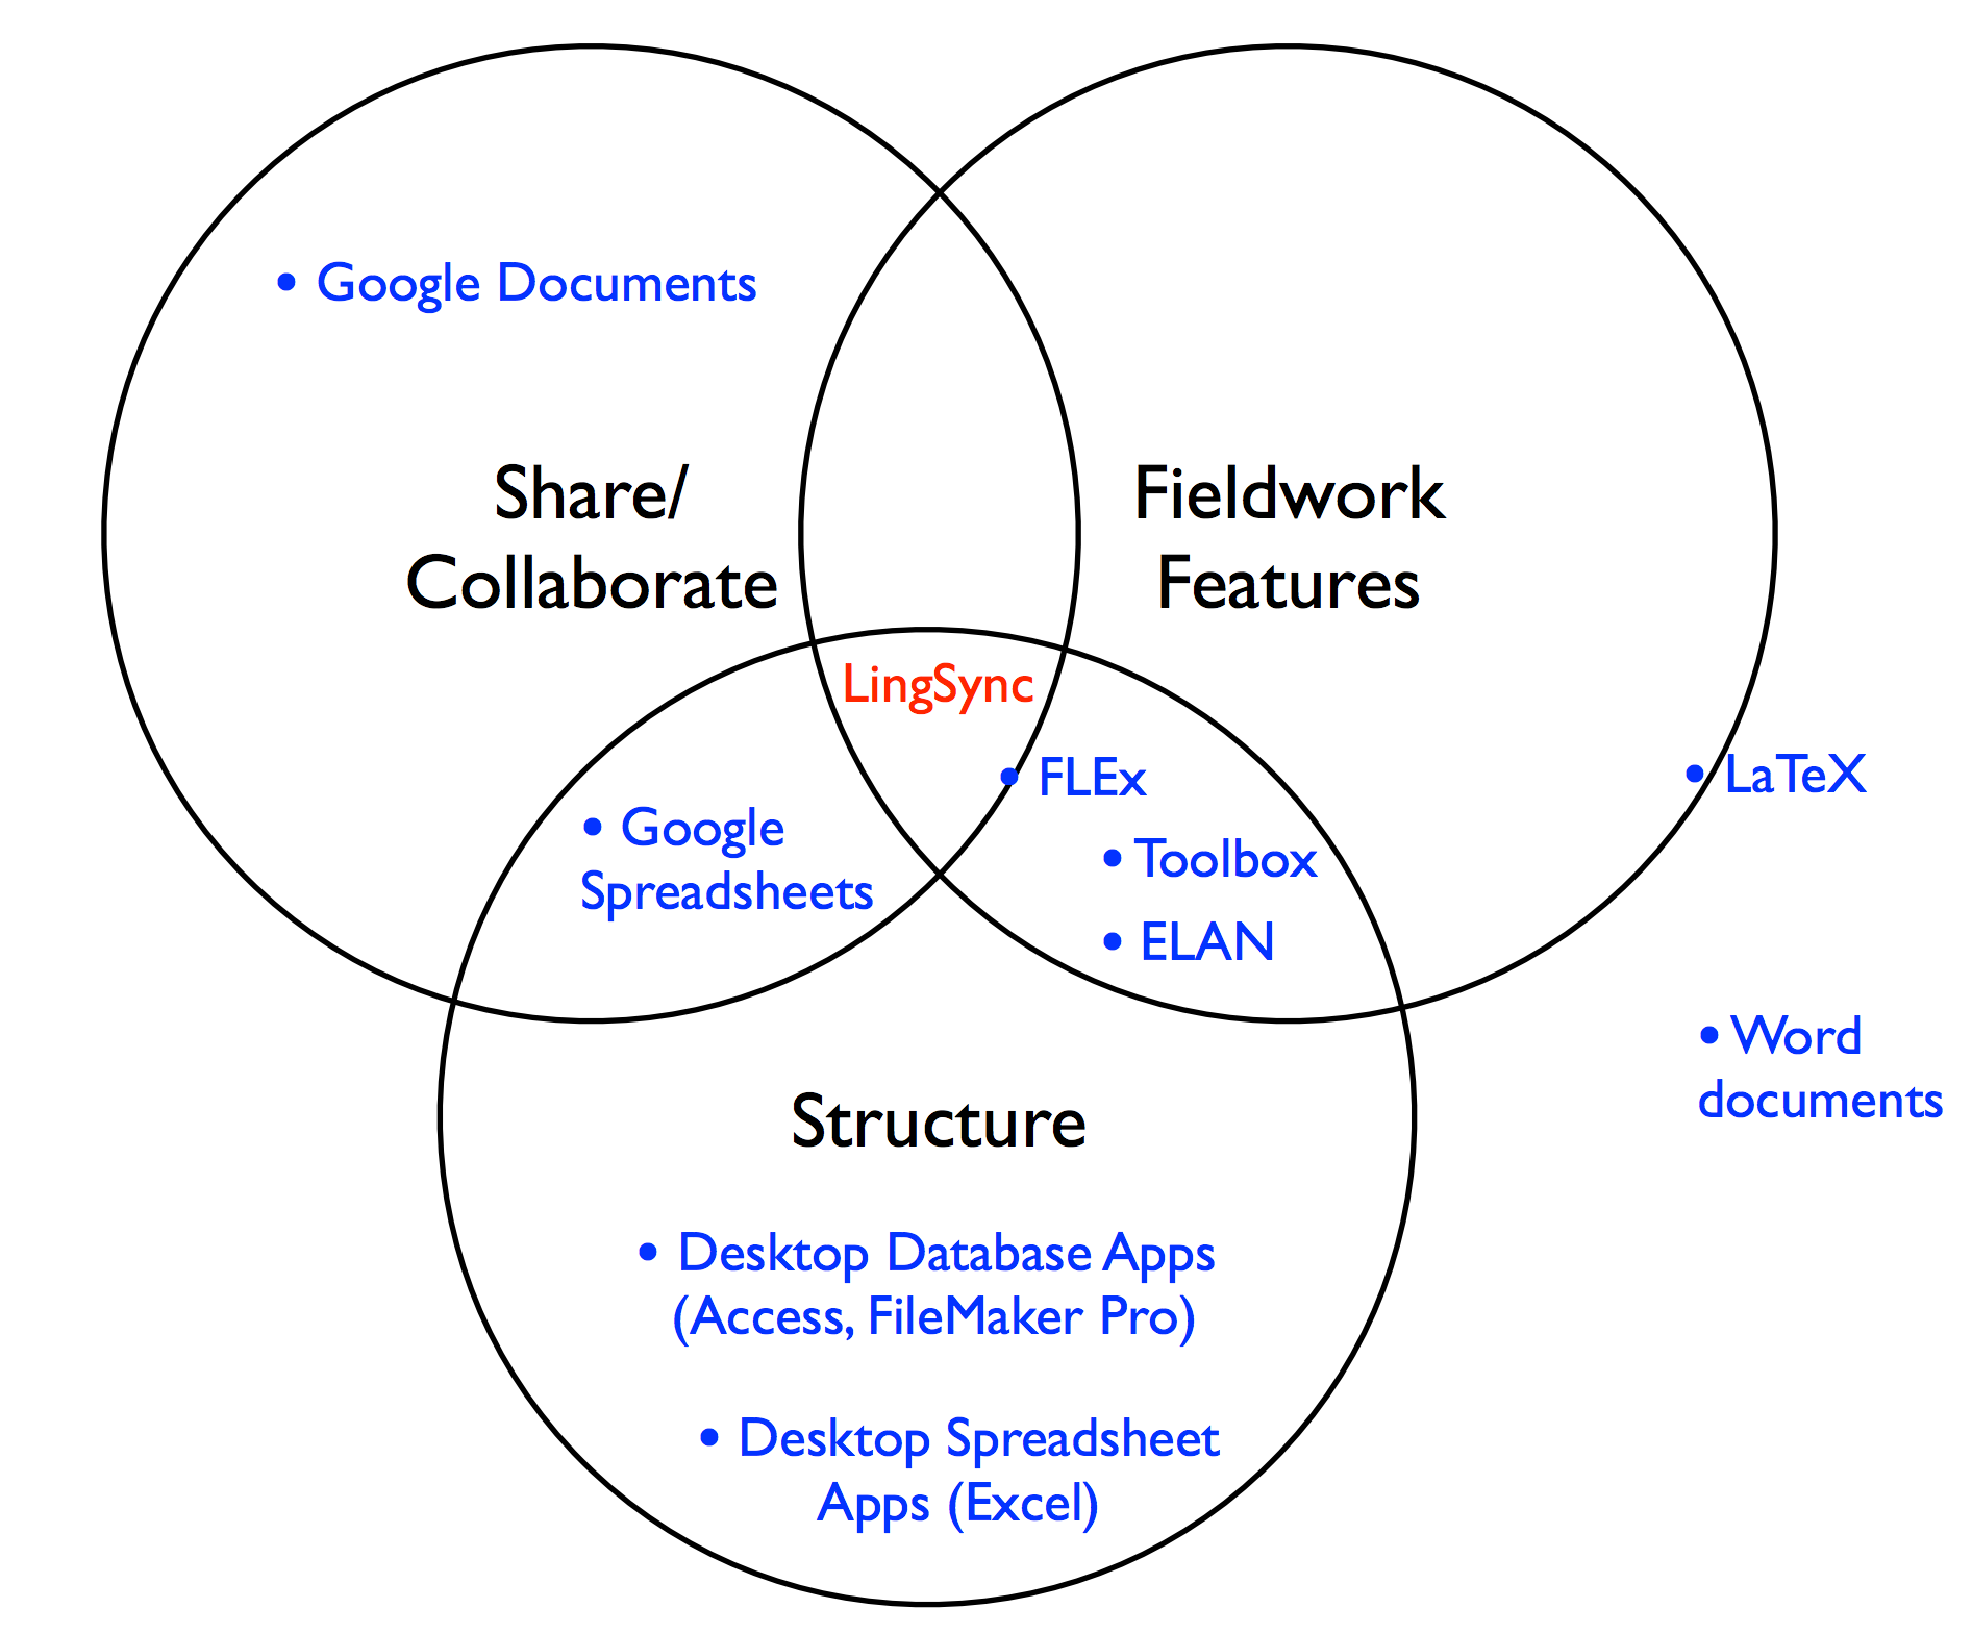
\includegraphics[width=3in]{../figures/other_software_sets}
\label{othersoftware}
\end{center}
\end{figure}

\note{Joel presents}
\end{frame}


\begin{frame}
%TODO will convert into latex diagrams once we are sure we want it.
\begin{figure}
\begin{center}
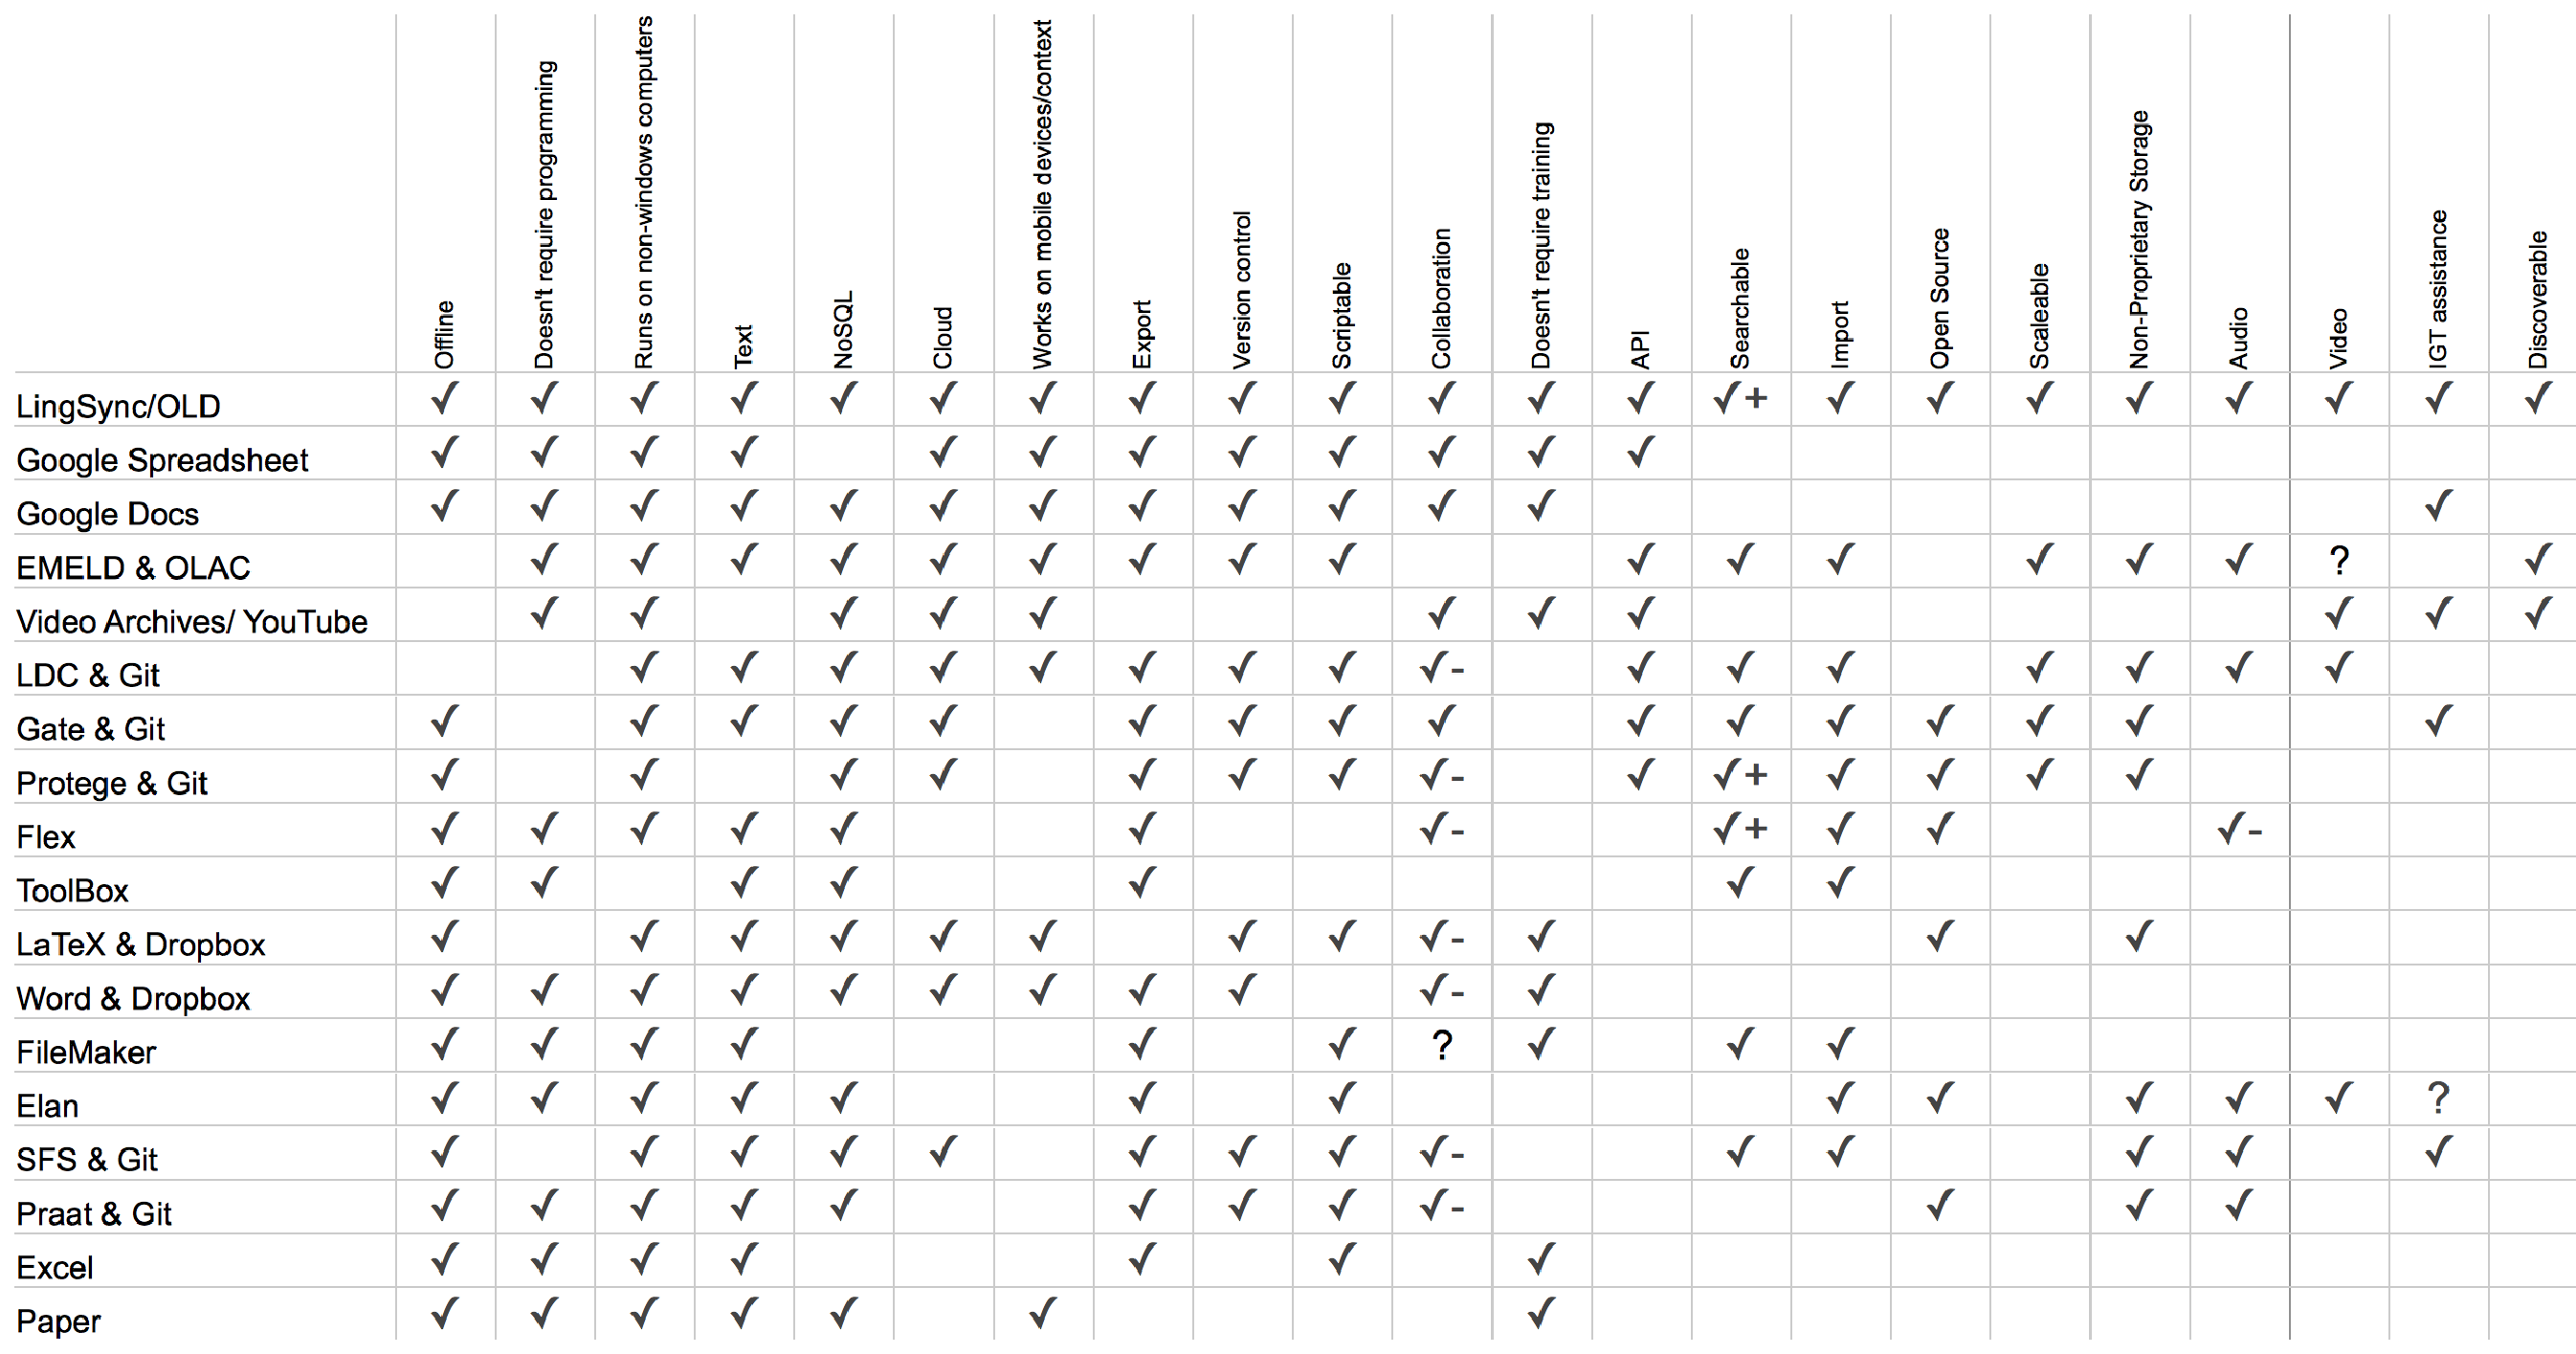
\includegraphics[width=3in]{../figures/other_software}
\caption{Many ad-hoc software combinations are used by teams.}
\label{allothersoftware}
\end{center}
\end{figure}

\note{Joel presents}
\end{frame}


\section[LingSync/OLD]{New models for data collection and management}
\subsection{LingSync}\label{sec:lingsync}



\begin{frame}
%TODO will convert into latex diagrams once we are sure we want it.
\begin{figure}
\begin{center}
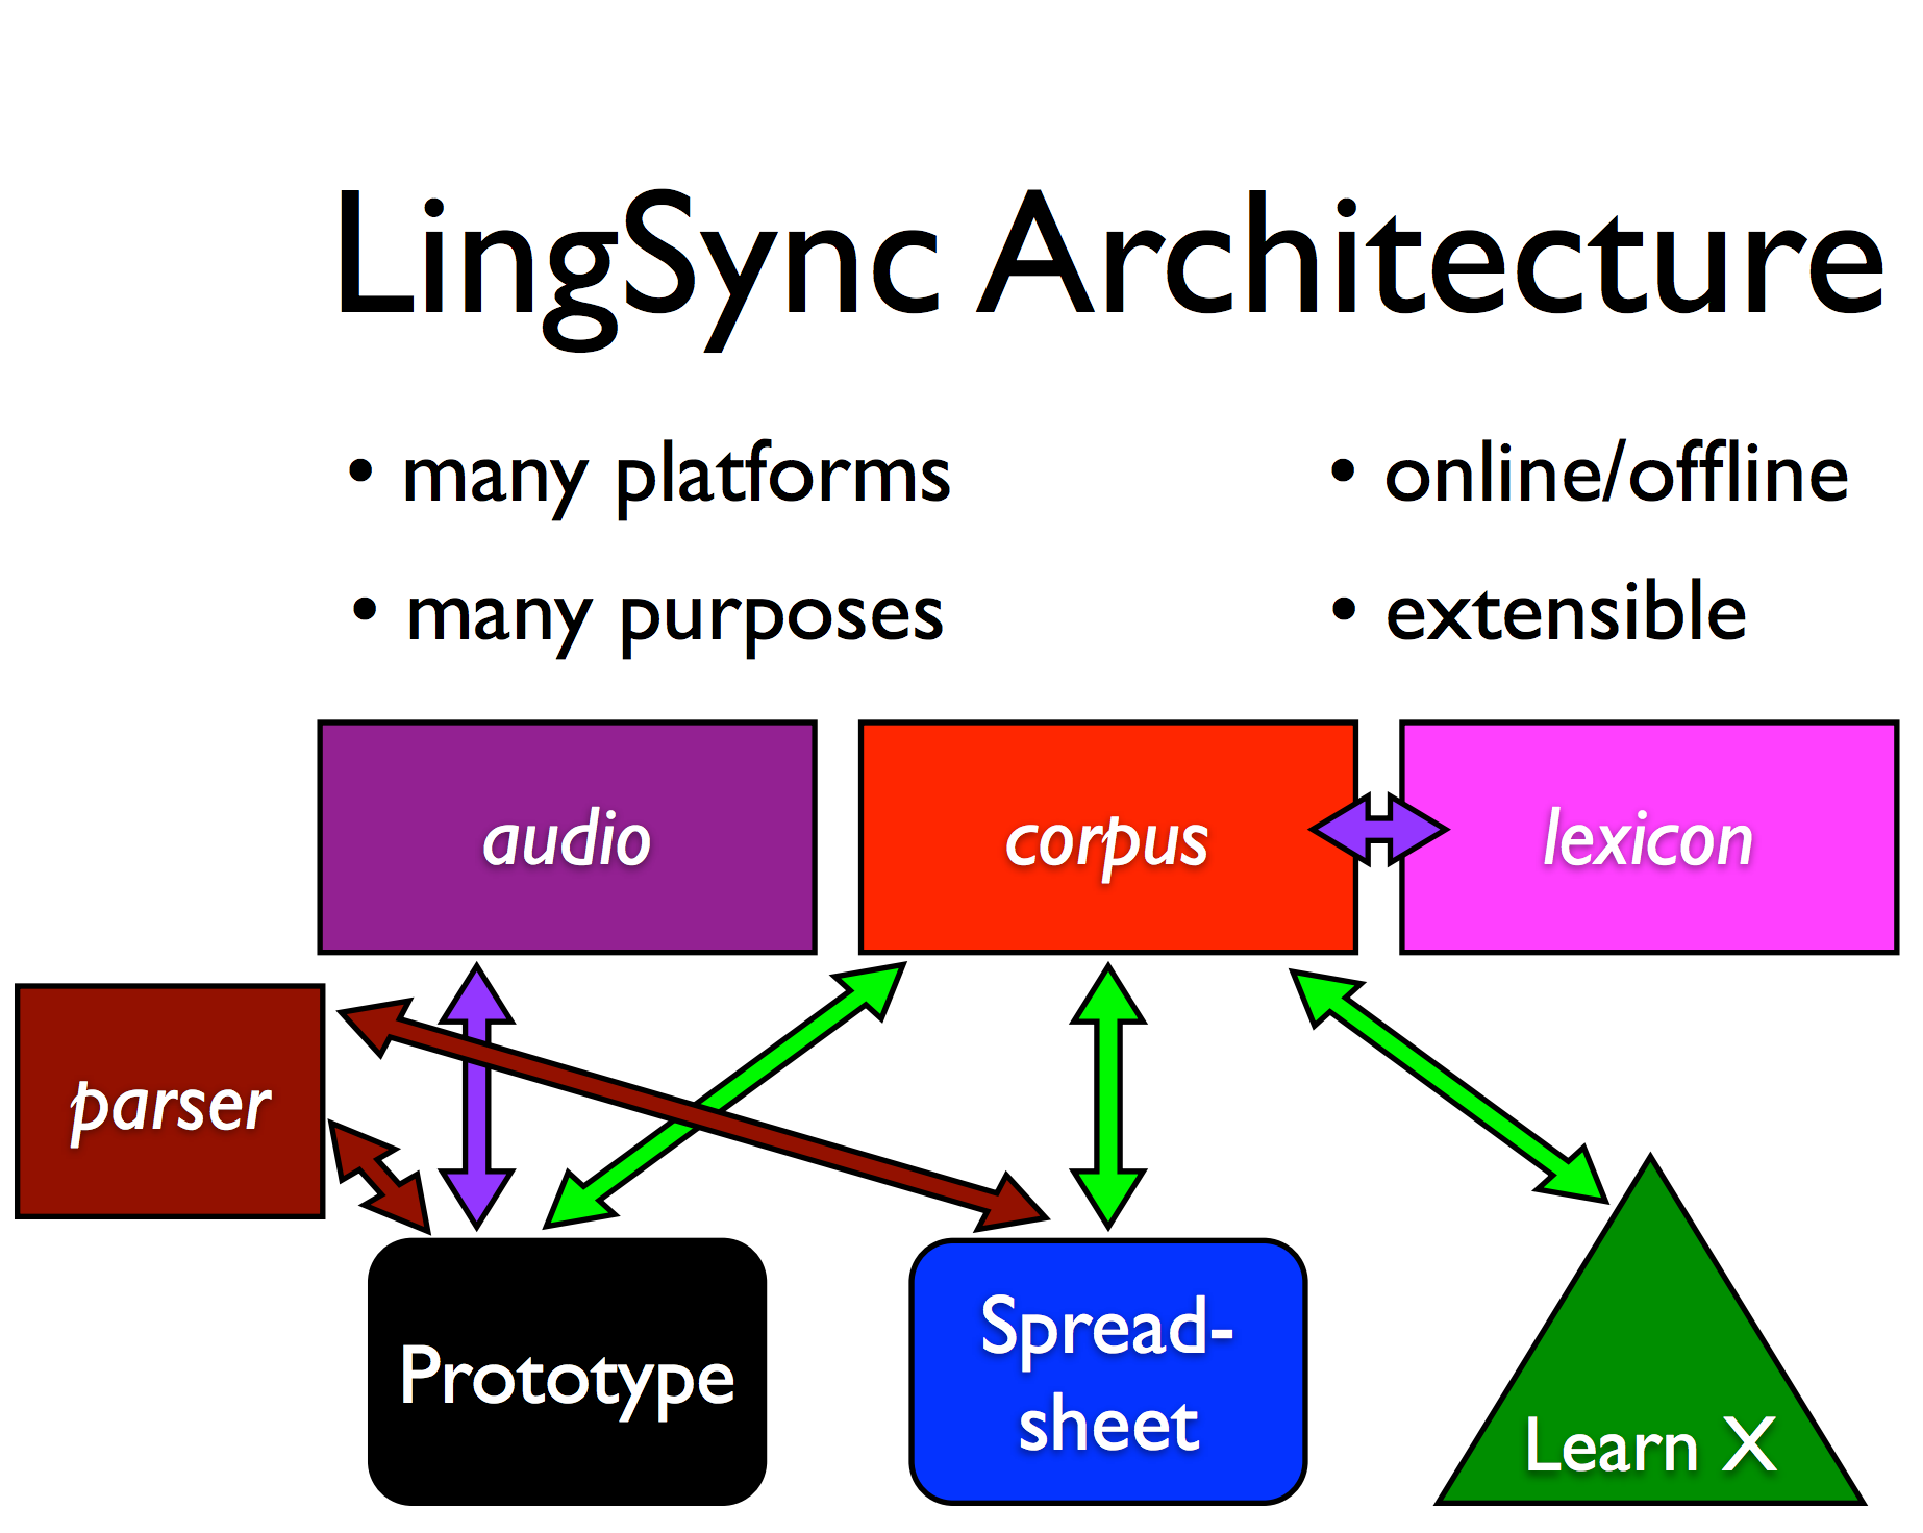
\includegraphics[width=3in]{../figures/architecture}
\label{lingsync:architecture}
\end{center}
\end{figure}
\note{Joel presents}
\end{frame}


\begin{frame}
%TODO will convert into latex diagrams once we are sure we want it.
\begin{figure}
\begin{center}
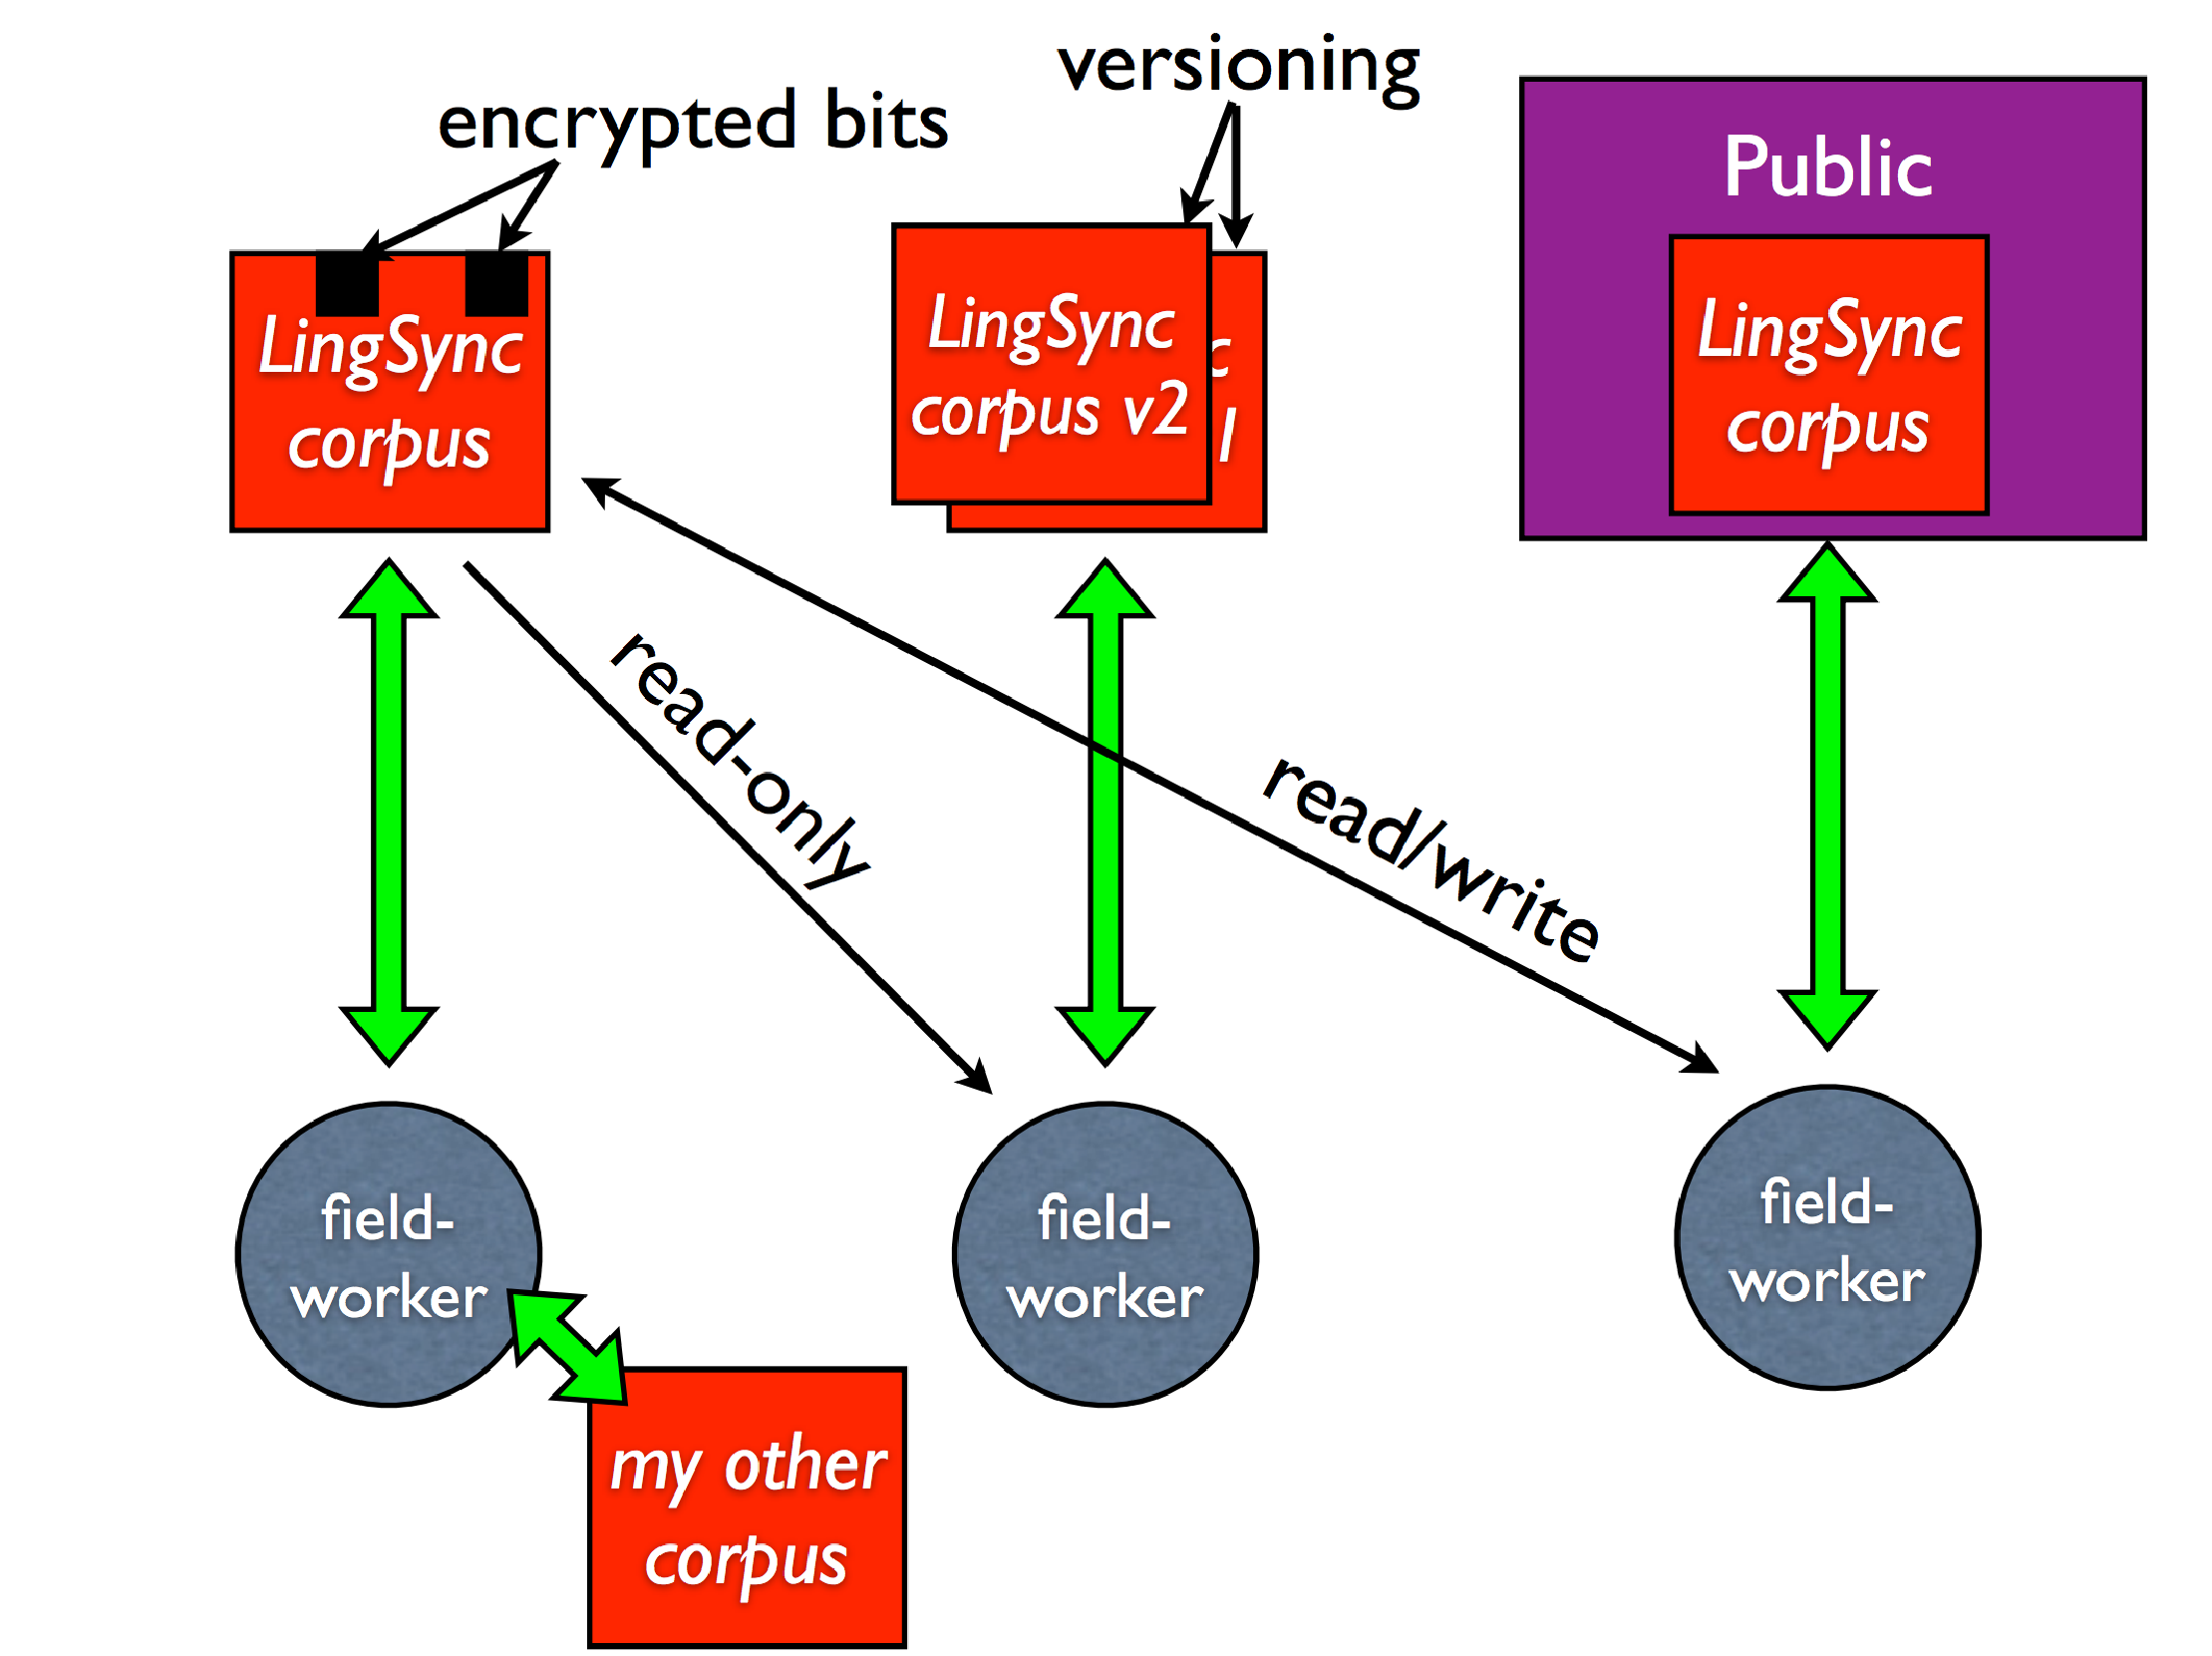
\includegraphics[width=3in]{../figures/corpora}
\label{lingsync:corpora}
\end{center}
\end{figure}
\note{Joel presents}
\end{frame}

%\subsection{OLD}\label{sec:old}

%\begin{frame}
%TODO Joel OLD
%\note{Joel presents}
%\end{frame}

%\subsection{LingSync/OLD}

\subsection{User adoption}

\begin{frame}

\begin{table}[h]
\begin{center}
\scriptsize
\begin{tabular}{lrrrr}
      \toprule
                     ~ &  Active & Investigating & In-active & Total\\
      \midrule
      Public Corpora  &       2 &   1 &   2 & 5 \\
      Private Corpora &      15 &  37 & 321 & 373\\
      Users           &      38 &  43 & 220 & 301 \\
      Documents & 13,408 & 2,763 & 4,541 &23,487\\
      Disk Size & 1GB & .9GB & 5.3GB& 7.2GB\\

      \bottomrule

\end{tabular}
\caption{Data in LingSync corpora (Feb 14, 2014). Active corpora: $>$300
activities; Investigating corpora: 300-10 activities; Active users: $>$100
activities; Investigating users: 100-10 activities.}
\label{lingsync-data}
 \end{center}
 \normalsize
\end{table}

\note{Joel presents}
\end{frame}

%
%\begin{frame}
%
%\begin{table}[h]
% \begin{center}
%     \scriptsize
%\begin{tabular}{lrrrrr}
%
%      \toprule
%      language &                     \emph{forms}  & texts & audio & GB   & speakers \\
%      \midrule
%      Blackfoot (\textit{bla}) &     8,847  & 171   & 2,057 & 3.8  & 3,350    \\ % 11,075 4047074461 bytes
%      Nata (\textit{ntk}) &          3,219  & 32    & 0     & 0    & 36,000   \\ % 3,251  0 bytes
%      Gitksan (\textit{git}) &       2,174  & 6     & 36    & 3.5  & 930      \\ % 2,216  3787227136 bytes
%      Okanagan (\textit{oka}) &      1,798  & 39    & 87    & 0.3  & 770      \\ % 1,924  349478912 bytes
%      Tlingit (\textit{tli}) &       1,521  & 32    & 107   & 12   & 630      \\ % 1,660  12906459136 bytes
%      Plains Cree (\textit{crk}) &   686    & 10    & 0     & 0    & 260      \\ % 696    0 bytes
%      Ktunaxa (\textit{kut}) &       467    & 33    & 112   & 0.2  & 106      \\ % 612    176128000 bytes
%      Coeur d'Alene (\textit{crd}) & 377    & 0     & 199   & 0.0  & 2        \\ % 576    28659712 bytes
%      Kwak'wala (\textit{kwk}) &     98     & 1     & 1     & 0.0  & 585      \\ % 100    7450624 bytes
%      TOTAL &                        19,187 & 324   & 2,599 & 19.8 &         \\ % 22,110 21302477981 bytes
%      \bottomrule
%
%\end{tabular}
%\caption{Data in OLD applications (Feb 14, 2014)}
%\label{old-data}
% \end{center}
% \normalsize
%\end{table}
%
%
%\note{Joel presents}
%\end{frame}

%\section[Data]{Using LingSync/OLD}\label{open-data}
%
%\begin{frame}
%Using LingSync/OLD
%\end{frame}


\section[Plugins]{Plugins \& Reusing existing tools and libraries}

\subsection{Audio}
%\subsubsection[Alignment]{Audio-transcription alignment}
%
%\begin{frame}
%
%\begin{figure}
%\begin{center}
%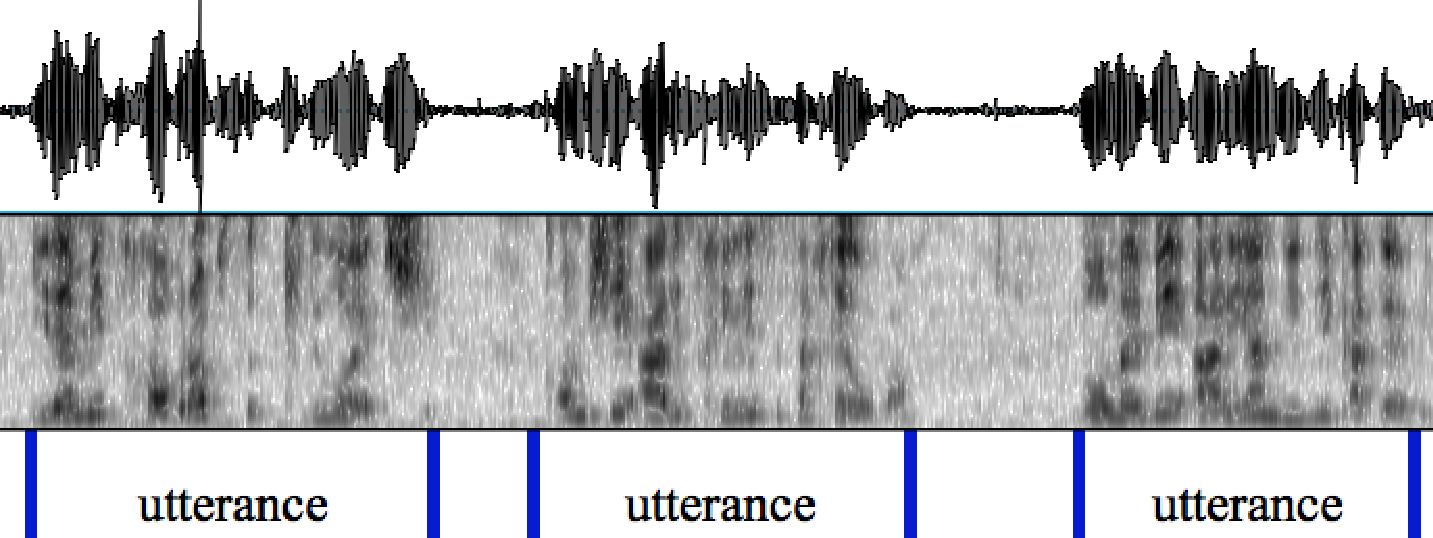
\includegraphics[width=3in]{../figures/utterance_extraction}
%\caption{Screenshot of the utterance extraction process which converts any
%audio/video into utterance intervals encoded either as \gls{json} or TextGrid using
%the PraatTextGridJS library.}
%\label{utterance_extraction_screenshot}
%\end{center}
%\end{figure}
%
%
%\note{Josh/Gina presents}
%\end{frame}


\subsubsection[ASR]{Speech Recognition for Information Retrieval}

\begin{frame}

\begin{figure}
\begin{center}
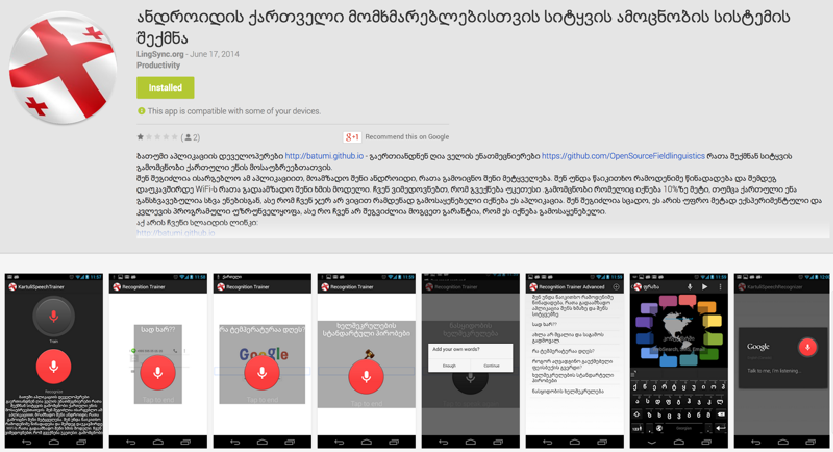
\includegraphics[width=3in]{../figures/kartuli_speech_recognition}
\caption{Screenshot of the Speech Recognition trainer}
\label{speech_recognition_screenshot}
\end{center}
\end{figure}

\note{Gina presents}
\end{frame}


\subsection{Morphology}



%\subsubsection[Existing]{Existing morphological parsers}
%
%\begin{frame}
%
%\begin{figure}
%\begin{center}
%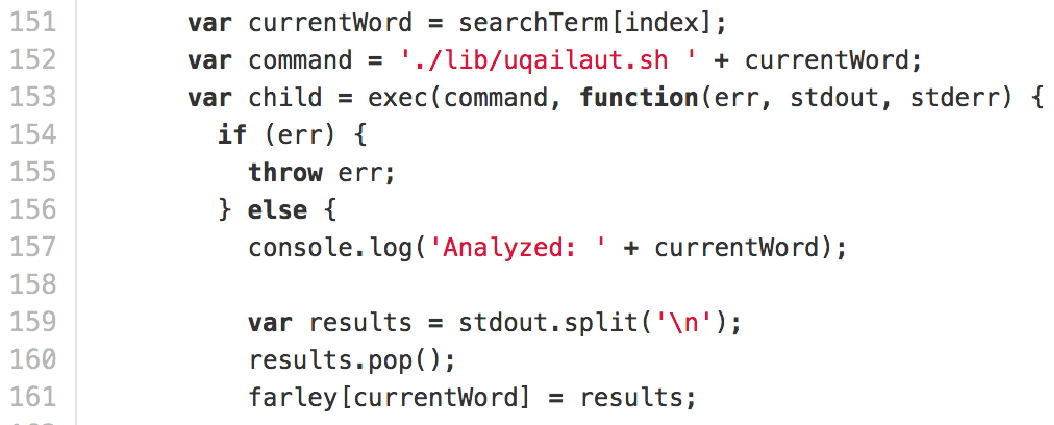
\includegraphics[width=2.5in]{../figures/farley}
%\\
%\includegraphics[width=2.5in]{../figures/inuktitut}
%\caption{Screenshot of Farley's Morphological Analyzer wrapped in a Node.js Web Service And offered in a HTML5 User Interface  }
%\label{speech_recognition_screenshot}
%\end{center}
%\end{figure}
%%\hspace{3in}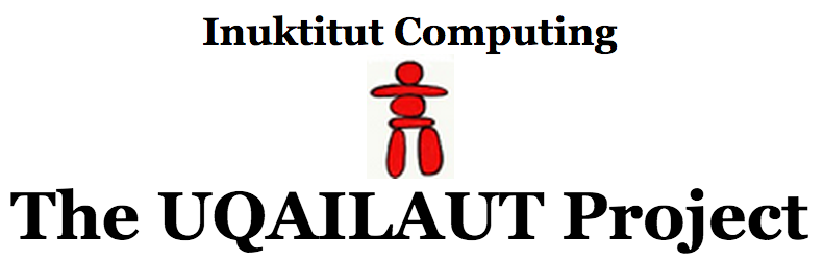
\includegraphics[width=1in]{../figures/inuktitut_computing}
%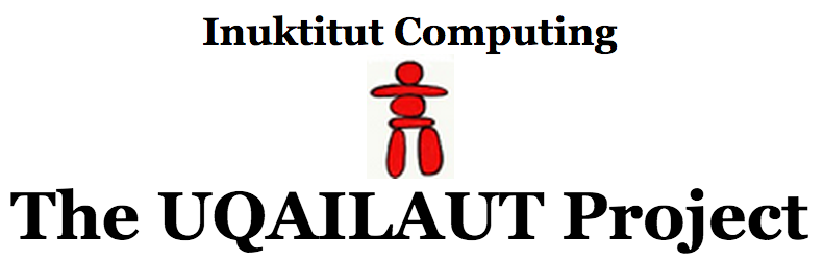
\includegraphics[width=1in]{../figures/inuktitut_computing}

%\note{Josh/Gina presents}
%\end{frame}




\subsubsection[Kartuli]{Semi-supervised seeded morphological parsers}

\begin{frame}


\begin{figure}
\begin{center}
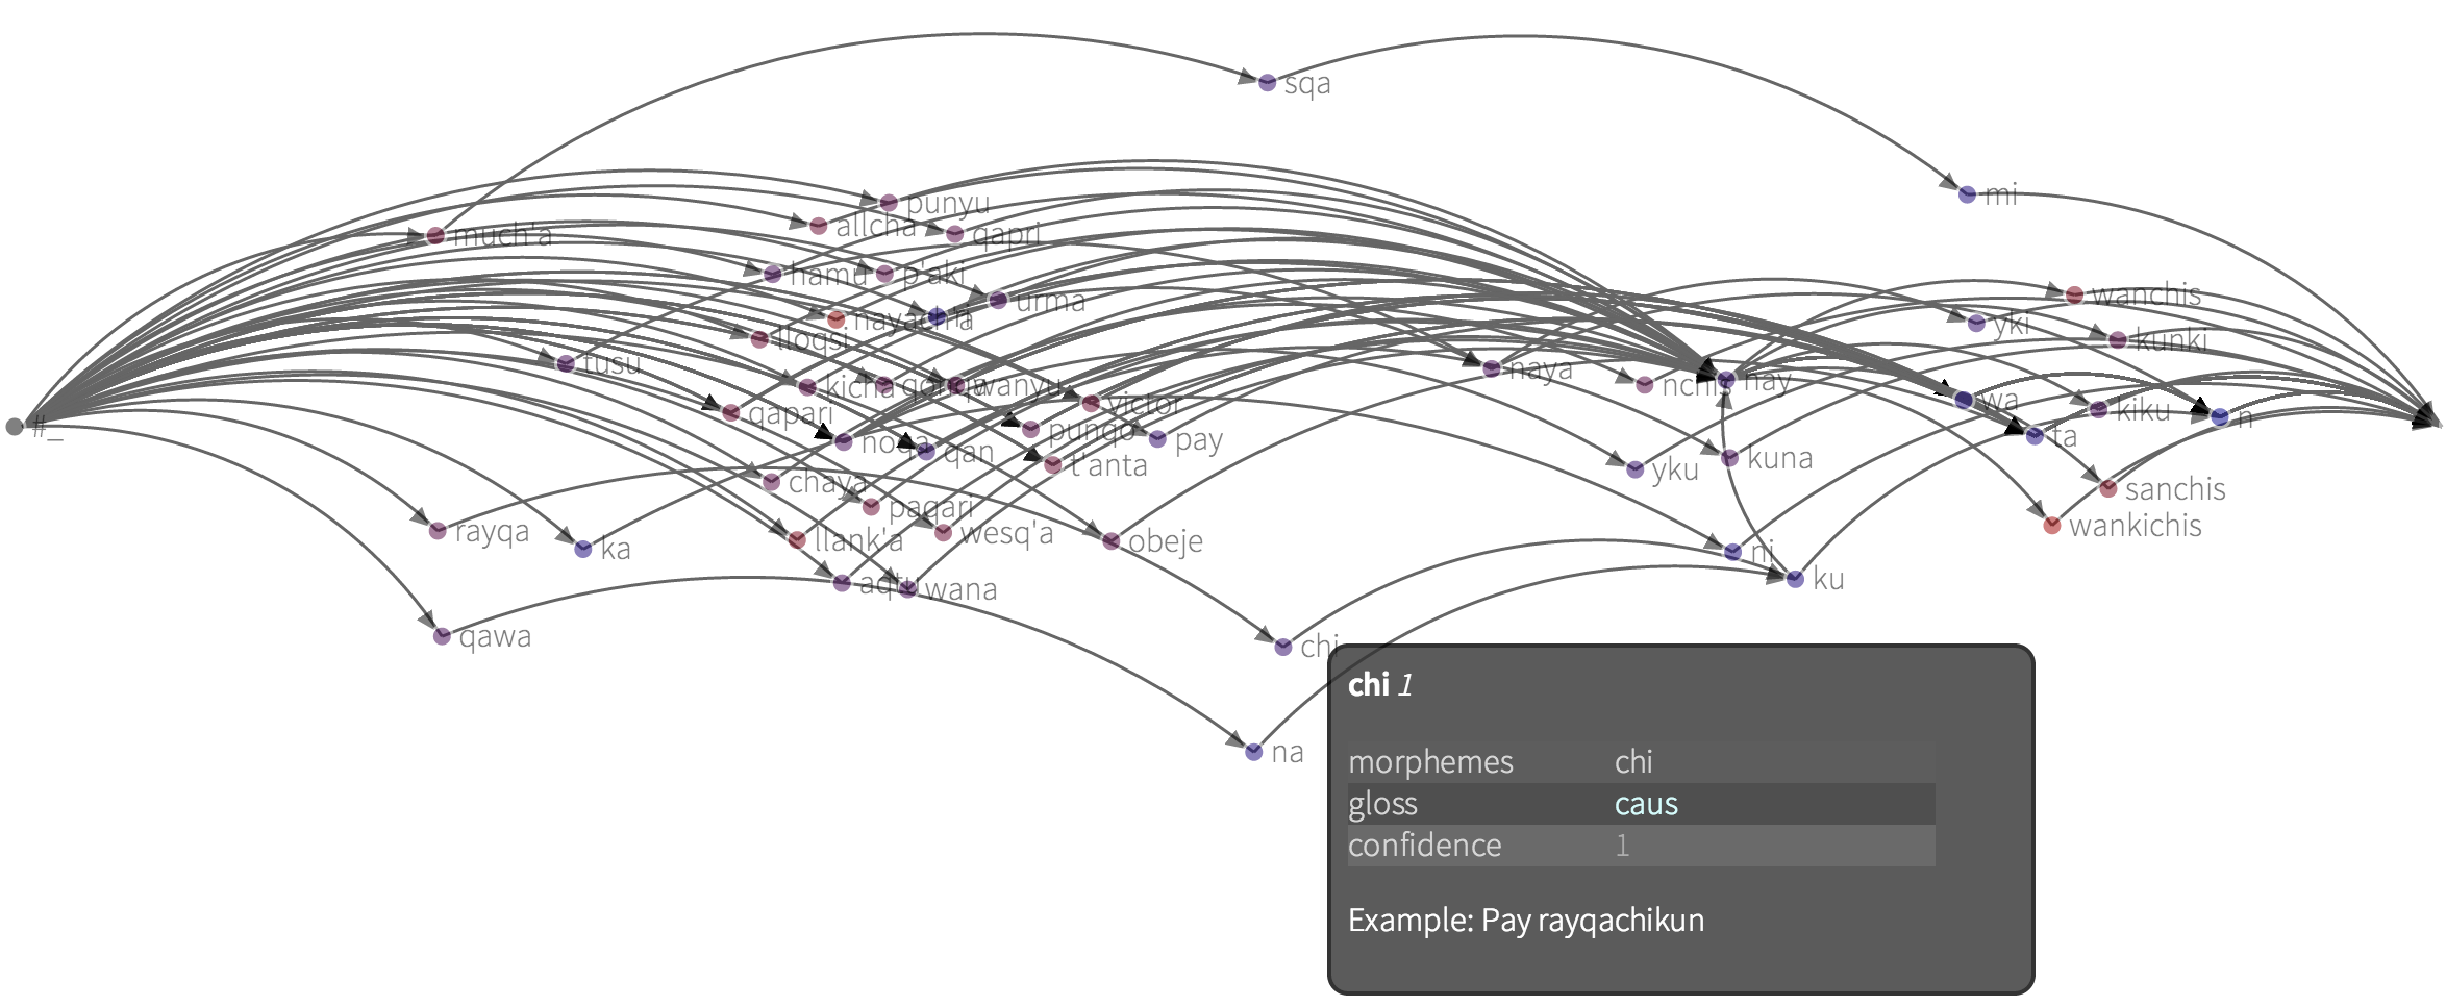
\includegraphics[width=3in]{../figures/lexicon_browser}\\
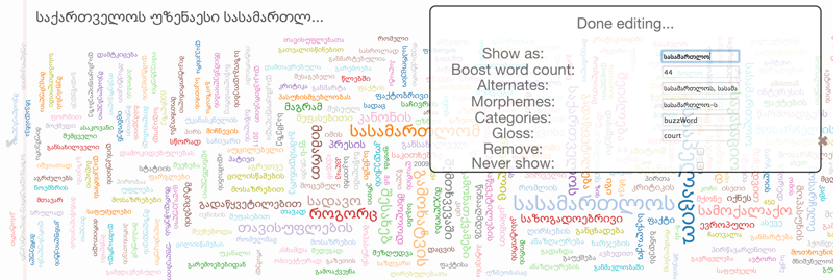
\includegraphics[width=3in]{../figures/lexicon_browser2}
\note{Screenshot of the Lexicon Browser, a web widget which lets users
browse words or relations between morphemes in their corpus, clean and add
declarative knowledge not found in the lexicon training process.}
\label{lexicon_browser_screenshot}
\end{center}
\end{figure}

\note{Gina presents}
\end{frame}



%
%\subsubsection[BlackFoot]{BlackFoot morphological parser}
%
%\begin{frame}
%TODO Joel BlackFoot morphological parser
%
%\note{Joel presents}
%\end{frame}
%
%
%\begin{frame}
%TODO Joel BlackFoot morphological parser
%
%\note{Joel presents}
%\end{frame}
%
%\begin{frame}
%TODO Joel BlackFoot morphological parser
%
%\note{Joel presents}
%\end{frame}



\section{The Take-Home}

\begin{frame}
\frametitle{Take Homes}
\begin{itemize}
\item High productivity requirements
\item All stakeholders, all devices, anywhere
\item Modular Web Services and Plugin Architecture
\item Open Source, Open Development, Open Data
\end{itemize}
\note{Joel presents}
\end{frame}

\section*{(Team)}

\begin{frame}
\frametitle{Acknowledgements}


Tobin Skinner, Elise McClay, Louisa Bielig, MaryEllen Cathcart, Theresa Deering, Yuliya Manyakina, Gretchen
McCulloch, Hisako Noguchi, Brian Doherty, Gay Hazan, Oriana Kilbourn, Kim Dan
Nguyen, Rakshit Majithiya, Mietta Lennes, Nivja de Jong, Ton Wempe, Kyle
Gorman, Curtis Mesher, Beso Beridze, Tornike Lasuridze, Zviadi Beradze, Rezo
Turmanidze, Jason Smith, Martin Gausby, Pablo Duboue, Xianli Sun, James Crippen,
Michael McAuliffe, Faryal
Abbassi, Farah Abbasi, Tamilla Paghava, Esma Chkhikvadze, Nina Gatenadze, and
Mari Mgeladze, Jessica Coon, Alan Bale and Michael
Wagner
~\\
~\\
SSHRC Connection Grant (\#611-2012-0001) \\
 SSHRC
Standard Research Grant (\#410-2011-2401)
\end{frame}



\begin{frame}
\tiny
\begin{itemize}
\item Dorothee Beermann and Pavel Mihaylov. 2012. TypeCraft collaborative databasing and resource sharing for linguists. Language Resources and Evaluation, pages 1?23.
\item Kenneth R Beesley and Lauri Karttunen. 2003. Finitestate morphology: Xerox tools and techniques. CSLI, Stanford.
\item H. Andrew Black and Gary F. Simons. 2006. The SIL FieldWorks Language Explorer approach to morphological parsing. In Computational Linguistics for Less-studied Languages: Proceedings of Texas Linguistics Society, Austin, TX.
\item Lynnika Butler and Heather van Volkinburg. 2007. Review of FieldWorks Language Explorer (FLEx). Language Documentation \& Conservation, 1(1):100?106.
\item MaryEllen Cathcart, Gina Cook, Theresa Deering, Yuliya Manyakina, Gretchen McCulloch, and Hisako Noguchi. 2012. LingSync: A free tool for creating and maintaining a shared database for communities, linguists and language learners. In Robert Henderson and Pablo Pablo, editors, Proceedings of FAMLi II: workshop on Corpus Approaches to Mayan Linguistics 2012, pages 247?250.
%\item N. Chomsky and M. Halle. 1968. The Sound Pattern of English. Harper \& Row, New York.
\item Jonathon E. Cihlar. 2008. Database development for language documentation: A case study in the Washo language. Master?s thesis, University of Chicago.
\item Gina Cook. 2009. Morphological parsing of Inuktitut. Ms, Concordia University, Faculty of Engineering and Computer Science.
\item David Costa. 2012. Surveying the sources on the Myaamia language. In Proceedings of the 2012 Myaamiaki Conference.
\item N.H. De Jong and T Wempe. 2009. Praat script to detect syllable nuclei and measure speech rate automatically. Behavior research methods, 41(2):385? 390.
\item Joel Dunham. 2014. Online Linguistic Database documentation. http://online-linguistic-database. readthedocs.org, March.
\item Benoit Farley. 2012. The Uqailaut project. //www.inuktitutcomputing.ca, January.
\item http: Scott Farrar. 2010. Review of TypeCraft. Language
\item Documentation \& Conservation, 4:6065.
\item Donald G. Frantz and Norma Jean Russell. 1995. Blackfoot Dictionary of Stems, Roots, and Affixes. Toronto: University of Toronto Press.
\item Donald G. Frantz. 1991. Blackfoot Grammar. Toronto: University of Toronto Press.
\item Andrew Garrett, Juliette Blevins, Lisa Conathan, Anna Jurgensen, Herman Leung, Adrienne Mamin, Rachel Maxson, Yoram Meroz, Mary Paster, Alysoun Quinby, William Richard, Ruth Rouvier, Kevin Ryan, and Tess Woo. 2001. The Yurok language project. http://linguistics.berkeley.edu/ yurok/index.php, January.
  \item Andrew Garrett, Susan Gehr, Line Mikkelsen, Nicholas Baier, Kayla Carpenter, Erin Donnelly, Matthew Faytak, Kelsey Neely, Melanie Redeye, Clare Sandy, Tammy Stark, Shane Bilowitz, Anna Currey, Kouros Falati, Nina Gliozzo, Morgan Jacobs, Erik Maier, Karie Moorman, Olga Pipko, Jeff Spingeld, and Whitney White. 2009. Karuk dictionary and texts. http://linguistics.berkeley.edu/karuk/links. php, January.
  \item Jeff Good. 2012a. Community collaboration in Africa: Experiences from northwest Cameroon. Language Documentation and Description, 11(1):2858.
  \item Jeff Good. 2012b. Valuing technology: Finding the linguistsplaceinanewtechnologicaluniverse.In Louanna Furbee and Lenore Grenoble, editors, Language documentation: Practice and values, pages 111131. Benjamins, Amsterdam.
  \item K David Harrison. 2007. When Languages Die: The Extinction of the Worlds Languages and the Erosion of Human Knowledge. Oxford University Press.
  \item M. Hulden. 2012. foma: finite state compiler and C library (documentation). https://code.google.com/p/ foma/w/list.
  \item George Ironstrack. 2012. Miloniteeheetaawi eehinki pimihkanaweeyankwi: Lets reflect on how far we have traveled. In Proceedings of the 2012 Myaamiaki Conference.
  \item Wesley Leonard. 2012. Your language isnt extinct: the role of Myaamia in Language Reclamation. In Proceedings of the 2012 Myaamiaki Conference.
  \item LingSync. 2012. WhitePaper. http: //OpenSourceFieldlinguistics.github.io/FieldDB/, January.
  \item Stuart Robinson, Greg Aumann, and Steven Bird. 2007. Managing fieldwork data with ToolBox and the Natural Language Toolkit. Language Documentation \& Conservation, 1(1):4457.
  \item Chris Rogers. 2010. Review of FieldWorks Language Explorer (FLEx) 3.0. Language Documentationation \& Conservation, 4:7884.
  \item R. Schroeter and N. Thieberger. 2006. EOPAS, the EthnoER online representation of interlinear text. In Sebastian Nordoff, editor, Sustainable Data from Digital Fieldwork. University of Sydney, Sydney.
  \item SIL International. 2013. Technical Notes on FieldWorks Send/Receive. http://fieldworks.sil.org/ wp-content/TechnicalDocs/, November.
  \item Nick Thieberger. 2012. Using language documentation data in a broader context. In Frank Seifart, Geoffrey Haig, Nikolaus P. Himmelmann, Dagmar Jung, Anna Margetts, and Paul Trilsbeek, editors, Potentials of Language Documentation: Methods, Analyses, and Utilization. University of Hawaii Press, Honolulu.
  \item Doug Troy and Andrew J. Strack. 2014. Metimankwiki kimehsoominaanaki we follow our ancestors trail: Sharing historical Myaamia language documents across myaamionki. In Proceedings of the 2014 Myaamiaki Conference.
  \item N. Weber. 2013. Accent and prosody in Blackfoot verbs. http://www.academia.edu/4250143/Accent and prosody in Blackfoot verbs.
  \item Alan Yu, Ryan Bochnak, Katie Franich, OzgeSarigul, Peter Snyder, Christina Weaver, Juan Bueno-Holle, Matt Faytak, Eric Morley, and Alice Rhomieux. 2005. The Washo project. http://washo.uchicago. edu/dictionary/dictionary.php, January.
  \item AlanYu,RyanBochnak,KatieFranich,OzgeSarigul, Peter Snyder, Christina Weaver, Juan Bueno-Holle, Matt Faytak, Eric Morley, and Alice Rhomieux. 2008. The Washo mobile lexicon. http://washo. uchicago.edu/mobile/, January.
\end{itemize}
\end{frame}


\end{document}
